\documentclass{kththesis}

\usepackage{blindtext} % This is just to get some nonsense text in this template, can be safely removed

\usepackage{csquotes} % Recommended by biblatex
\usepackage{biblatex}
\addbibresource{references.bib} % The file containing our references, in BibTeX format

%added by me:
\usepackage{xcolor}
\usepackage{color}
\usepackage{amsmath,float}
\usepackage{caption}
\captionsetup[figure]{labelfont=bf}
\usepackage{amsthm}
\theoremstyle{definition}
\newtheorem{definition}{Definition}[section]
\newtheorem{hyp}{Hypothesis}
\newtheorem{RQ}{Research Question}[section]

\usepackage{graphicx}

%for clickable hyperlinks
%colors for different links
\usepackage{hyperref}
\hypersetup{
    colorlinks,
    linkcolor={red!50!black},
    citecolor={blue!50!black},
    urlcolor={blue!80!black}
}

\usepackage{cleveref}

\graphicspath{{Imgs/}}

\title{Competitive self-playing reinforcement learning agents used in the Nordic stock market, to understand market microstructure}

\alttitle{Reinforcement learning agenter i den nordiska aktiemarknaden, för att förstå marknadens mikrostruktur }
\author{Marcus Elwin}
\email{elwi@kth.se}
\supervisor{Hamid Reza Faragardi}
\examiner{Elena Troubitsyna}
\programme{Master of Science in Machine Learning}
\school{School of Electrical Engineering and Computer Science}
\date{\today}



\begin{document}


% Frontmatter includes the titlepage, abstracts and table-of-contents
\frontmatter

\titlepage

\begin{abstract}
  English abstract goes here.

\end{abstract}


\begin{otherlanguage}{swedish}
  \begin{abstract}
    Svensk sammanfattning
  \end{abstract}
\end{otherlanguage}


\tableofcontents


% Mainmatter is where the actual contents of the thesis goes
\mainmatter


\chapter{Introduction}

%We use the \emph{biblatex} package to handle our references.  We therefore use the
%command \texttt{parencite} to get a reference in parenthesis, like this
%\parencite{heisenberg2015}.  It is also possible to include the author
%as part of the sentence using \texttt{textcite}, like talking about
%the work of \textcite{einstein2016}.

\section{Background}
Modern financial markets such as NASDAQ, CME and NYSE have all been effected by the rise and presence of \textit{Algorithmic Trading} and \textit{High-Frequency Trading} (HFT).  Where both types of trading consists in using computer programs to implement investment and trading strategies \parencite{abergel2012market}. These types of strategies have according to \textcite{abergel2012market, o2015high} raised various questions about there effects on the financial markets. Mainly in areas as: \textit{liquidity, volatility, price discovery, systematic risk, manipulation} and \textit{market organization}. Where a quite recent example of the proposed effect of algorithmic trading and HFT on financial markets is \textit{the Flash Crash} in the 6th of May 2010. Where in the course of 30 minutes U.S. stock market indices, stock-index futures, options, and exchange-traded funds. Experienced a sudden price drop of more than five percent,followed by a rapid rebound \parencite{kirilenko2011flash,kirilenko2017flash}. See an illustration of this in \autoref{fig:1}.
\newline
\newline
Trading in the financial market can be seen as a search problem, which depends on market structure \parencite{abergel2012market}. \textit{Market microstructure} is a branch of economics, where one tries to understand trading dynamics on the financial market on a micro level \parencite{o1995market, hasbrouck2007empirical}. Market microstructure theory is used by regulators, traders and organizers of financial markets. in order to make a profit or create more transparent and efficient markets. Where a recent regulation with the purpose of making markets more transparent and efficient is \textit{Markets in Financial Instruments Directive} (MiFID) II \parencite{busch2016mifid}.

\begin{figure}[ht]
    \centering
    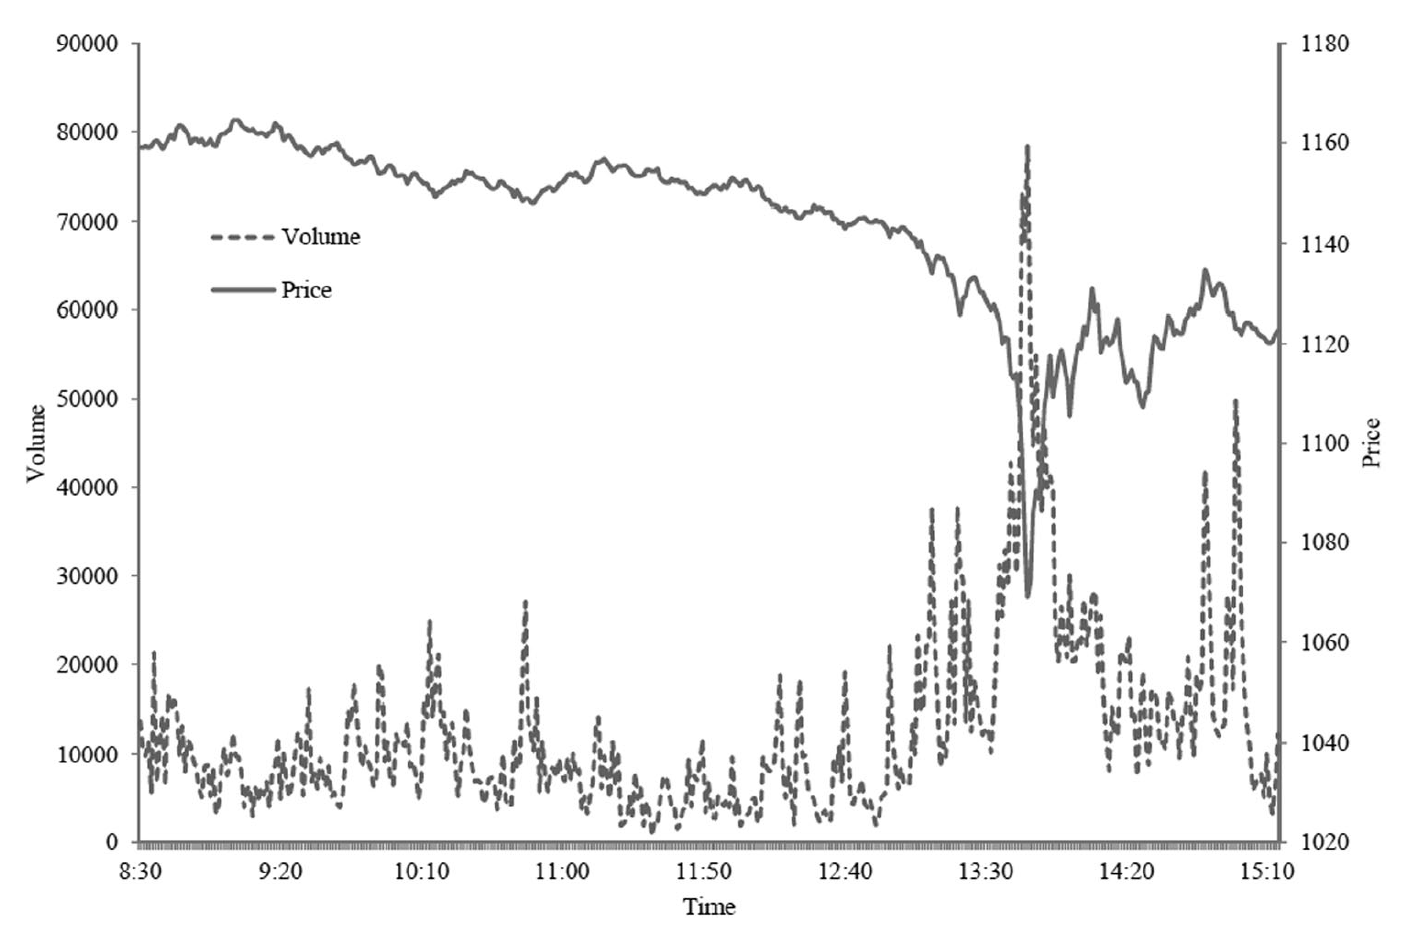
\includegraphics[scale=.7]{flashcrash.PNG}
    \caption{Minute-by-minute transaction prices and trading volume on E-mini S\& P futures contracts during the flash crash, between 8:30 to 15:15. Notice the distinct drop and rebound at the end of the day. Source: \textcite{kirilenko2017flash} }
    \label{fig:1}
\end{figure}

However as mentioned by \textcite{o2015high} due to HFT and algoritmic trading. Learning models and empirical models used in market microstructure in the past are deficient and may not longer be appropriate. Which calls for the use of new more capable methods. Where \textit{Reinforcement Learning} and other machine learning methods are of great interest. Machine learning and AI has been used in a financial setting for some time, and has become ubiquitous in finance today. Mainly due to the abundance of available data and computing power. 
\newline
\newline
Where recent achievements for the use of Reinforcement Learning has been seen in the game Go with \textit{AlphaGo, AlphaGoZero} \parencite{silver2016mastering} programs being able to win over esteemed Go champions. More complicated strategic games as Star Craft has also seen succesfull applications of reinforcment learning \parencite{vinyals2017starcraft}. Therefore the focus of this thesis will be to examine the possibility of using deep reinforcement learning and competitive self-play. In order to understand the market microstructure on a simulated Nordic stock market.

%need to work with
\section{Research Question}
The research question for this thesis is shown below:

\begin{RQ}
Will trading dynamics such as the bid-ask spread clustering, optimal trade execution and optimal inventory costs be exhibited \& learned by reinforcement learning agents using competitive self-play on a simulated Nordic stock market.
\end{RQ}


 



\section{Problem}

\section{Aim}

\section{Objective}

\section{Delimitation}

\section{Disposition}

%The student displays knowledge of theoretical background and previous related work (significant literature is mentioned and relevant material is used).

The background is coherent and relevant.
\chapter{Background}
In this chapter relevant theory is presented in order to give the reader a good overview of the fields study during the pre-study that are relevant for the thesis. We begin with .. and finally end with a section on previous related work.

%Necessary
\section{Modern Financial Markets}

\subsection{Participants}
A \textit{market} is the place where traders gather to trade \parencite{harris2003trading} different types of instruments as common stocks, bonds, futures, options, derivatives and foreign exchange rates just to mention a few.
Looking at today's financial markets
\textcite{cartea2015algorithmic} broadly categories three primary classes of traders (or strategies) that partake in the market:
\begin{itemize}
    \item \textbf{Fundamental traders:} those who are driven by economic fundamentals outside the exchange.
    \item \textbf{Informed traders:} traders who profit from leveraging information not reflected in market prices and trading assets in the hope of their increase or decrease in value.
    \item \textbf{Market Makers:} professional trader who profit from facilitating exchange in a particular asset and exploit their skills in executing trades.
\end{itemize}

\subsection{Liquidity}
One common measure to characterize financial markets are \textit{liquidity}. Liquidity impounds the usual economic concept of \textit{elasticity}, and liquidity is sometimes defined as 'depth, breadth and resiliency' \parencite{hasbrouck2007empirical}.

\subsection{Orderbook}

%mention what it is, some strategies, and how it effect modern markets
\subsection{Algorithmic and High-Frequency Trading}
High frequency trading is a term used to describe a large diverse set of activities and behaviors \parencite{o2015high}. Where some of the main characteristics for high frequency traders are: (i) use of \textit{high-speed} and sophisticated programs for \textit{generating, executing} and \textit{routing} orders, (ii) use of \textit{co-location} to minimize \textit{latency}, (iii) very short time frames for their positions, (iv) submission of numerous orders that are cancelled shortly and (v) ending the day with almost flat positions.

%Ho stoll model for invetory market

%GM

% Daz model for informed traders

% Real market with matching engine e.g. parity
\section{Market Microstructure}
\textit{Market microstructure} is the study of the process and outcomes of exchanging assets under implicit trading rules as mentioned in\textcite{o1995market}

\section{Artificial Financial Markets}


\section{Reinforcement Learning}

\subsection{The Main Concepts}
Reinforcement learning (RL) is learning what to do i.e. map situations to actions, in order to maximize a numerical reward function \parencite{sutton1998reinforcement}. Which is quite different from other machine learning methods based on \textit{supervised} or \textit{unsupervised} learning, where one in fact have the true labels or not.

\subsection{Exploration versus Exploitation}
In reinforcement learning we have a trade-off between \textit{exploration} and \textit{exploitation}. Where exploration refers to taking actions, that come from the current best version of the learned policy. Exploration instead is concerned with taking more actions to obtain more training data \parencite{goodfellow2016deep}. Where the dilemma is that neither exploration nor exploitation can be pursued exclusively without failing at the task \parencite{sutton1998reinforcement}.

\subsection{Algorithms \& Learning in RL}
One can characterize RL problems into two main classes: \textit{prediction} and \textit{control} where each is followed by different approaches as \textit{value iteration, policy iteration} and \textit{policy search} \parencite{szepesvari2009algorithms}. These different approaches uses different algorithms 

\subsection{Competitive Self-Play}

%mention where it has been succesfully used and show the need of the application that we want to use here for the thesis
\subsection{Reinforcement Learning in Market Microstructure}


%necessary?
\section{Tree Search}

\subsection{MinMax}

\subsection{Monte Carlo Tree Search (MCTS)}

%own chapter?
\section{Related Work}


\chapter{Methods}

\chapter{Experiments}

\chapter{Results}

\chapter{Discussion \& Conclusions}

\printbibliography[heading=bibintoc] % Print the bibliography (and make it appear in the table of contents)

\appendix

\chapter{Unnecessary Appended Material}

\end{document}
